\section{Results}

We validate our enhanced dataset against a comprehensive set of official statistics and compare its performance to both the original CPS and PUF datasets. Our validation metrics cover 570 distinct targets spanning demographic totals, program participation rates, and detailed income components across the distribution.

\subsection{Validation Against Administrative Totals}

The enhanced CPS (ECPS) shows substantial improvements over both of its source datasets. When comparing absolute relative errors across all targets, the ECPS outperforms:
\begin{itemize}
    \item The Census Bureau's CPS in 63.0\% of targets
    \item The IRS Public Use File in 70.7\% of targets
\end{itemize}

These improvements are particularly notable because they demonstrate that our enhancement methodology successfully combines the strengths of both source datasets while mitigating their individual weaknesses. The CPS excels at demographic representation but struggles with income reporting, particularly at the top of the distribution. Conversely, the PUF captures tax-related variables well but lacks demographic detail. Our enhanced dataset achieves better accuracy than either source across most metrics.

\subsection{Distribution of Improvements}

To assess the magnitude and consistency of these improvements, we calculate the relative error change under the ECPS compared to the better performing of the CPS or PUF for each target. The distribution of these improvements shows that:

\begin{itemize}
    \item Most improvements cluster between 5-15\% reduction in relative error
    \item Some targets see improvements exceeding 50\% reduction in error
    \item Very few targets show degraded performance compared to the source datasets
\end{itemize}

A detailed, interactive validation dashboard showing performance across all targets is maintained at \url{https://policyengine.github.io/policyengine-us-data/validation.html} and updates automatically with each dataset revision. This transparency allows users to assess the dataset's strengths and limitations for their specific use cases. See Figure \ref{fig:ecps_vs_cps_puf} for a visualization of the distribution of improvements.

\begin{figure}[h]
    \centering
    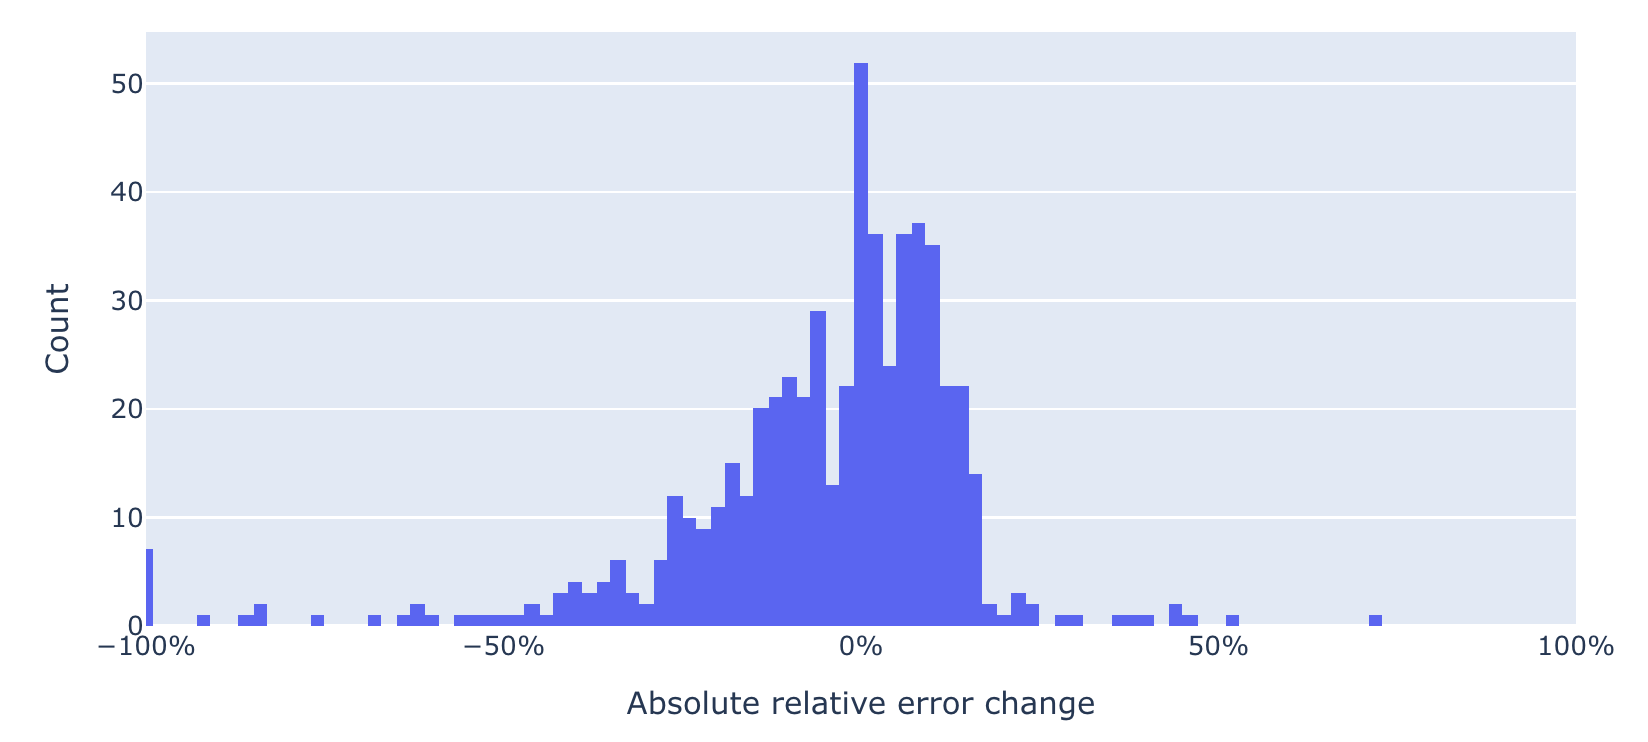
\includegraphics[width=\textwidth]{figures/ecps_vs_cps_puf.png}
    \caption{Relative error change under the ECPS compared to the better performing of the CPS or PUF for each target.}
    \label{fig:ecps_vs_cps_puf}
\end{figure}
